\documentclass[aspectratio=169]{beamer}

\usetheme{Boadilla}
\usefonttheme{professionalfonts}
\setbeamertemplate{navigation symbols}{}
\setbeamertemplate{itemize items}[circle]
\setbeamertemplate{enumerate items}[default]
\setbeamertemplate{headline}{}

\usepackage[utf8]{inputenc}
\usepackage[T1]{fontenc}
\usepackage{lmodern}
\usepackage{amsmath}
\usepackage{booktabs}
\usepackage{tabularx}
\usepackage{array}
\usepackage{hyperref}
\usepackage[strings]{underscore}
\usepackage{listings}
\usepackage{tikz}
\usetikzlibrary{arrows.meta,positioning,fit,calc,shapes.geometric}
\usepackage{xcolor}

\definecolor{courseblue}{HTML}{12355B}
\definecolor{coursegold}{HTML}{C98A2E}
\definecolor{courseice}{HTML}{EEF3F8}
\definecolor{coursegreen}{HTML}{2F6B4F}
\definecolor{coursegray}{HTML}{4B5563}
\definecolor{codebg}{HTML}{F7F9FC}
\definecolor{codecomment}{HTML}{5E6C84}
\definecolor{codestring}{HTML}{0B6E4F}

\setbeamercolor{palette primary}{bg=courseblue,fg=white}
\setbeamercolor{palette secondary}{bg=coursegold,fg=white}
\setbeamercolor{palette tertiary}{bg=courseblue,fg=white}
\setbeamercolor{palette quaternary}{bg=coursegold,fg=white}
\setbeamercolor{structure}{fg=courseblue}
\setbeamercolor{frametitle}{bg=courseice,fg=courseblue}
\setbeamercolor{title}{fg=courseblue}
\setbeamercolor{block title}{bg=courseblue,fg=white}
\setbeamercolor{block body}{bg=courseice,fg=black}
\setbeamercolor{normal text}{fg=black,bg=white}
\setbeamercolor{alerted text}{fg=coursegold}

\setbeamerfont{footline}{size=\scriptsize}

\setbeamertemplate{footline}{
  \leavevmode
  \hbox{
    \begin{beamercolorbox}[wd=.33\paperwidth,ht=2.8ex,dp=1.2ex,leftskip=0.8em]{palette primary}%
      University of Trieste
    \end{beamercolorbox}%
    \begin{beamercolorbox}[wd=.49\paperwidth,ht=2.8ex,dp=1.2ex,center]{palette tertiary}%
      \coursename{} \textbar{} \coursecode
    \end{beamercolorbox}%
    \begin{beamercolorbox}[wd=.18\paperwidth,ht=2.8ex,dp=1.2ex,rightskip=0.8em plus1fil]{palette secondary}%
      \insertframenumber{} / \inserttotalframenumber
    \end{beamercolorbox}%
  }
}

\hypersetup{
  colorlinks=true,
  linkcolor=courseblue,
  urlcolor=coursegreen
}

\lstdefinestyle{coursepython}{
  language=Python,
  basicstyle=\ttfamily\footnotesize,
  keywordstyle=\color{courseblue}\bfseries,
  commentstyle=\color{codecomment}\itshape,
  stringstyle=\color{codestring},
  showstringspaces=false,
  columns=fullflexible,
  keepspaces=true,
  frame=single,
  framerule=0.6pt,
  rulecolor=\color{courseblue},
  backgroundcolor=\color{codebg},
  xleftmargin=0.4em,
  xrightmargin=0.4em,
  aboveskip=0.4em,
  belowskip=0.2em
}

\newcommand{\coursename}{Data-driven Systems Engineering}
\newcommand{\coursecode}{440MI / 305SM}
\newcommand{\coursefooter}{}

\newcommand{\learninggoals}[1]{
  \begin{block}{Learning goals}
  #1
  \end{block}
}

\newcommand{\repoactivity}[1]{
  \begin{block}{Repo activity}
  #1
  \end{block}
}

\newcommand{\readinglist}[1]{
  \begin{block}{Papers and materials}
  {\footnotesize #1}
  \end{block}
}

\newcommand{\coursecontextframe}[5]{
  \begin{frame}{Course Map and Running Cases}
  \centering
  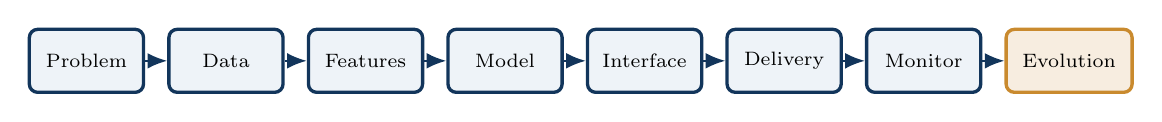
\begin{tikzpicture}[node distance=0.28cm]
  \node[flowbox, minimum width=1.45cm, minimum height=0.8cm] (problem) {\scriptsize Problem};
  \node[flowbox, minimum width=1.45cm, minimum height=0.8cm, right=of problem] (data) {\scriptsize Data};
  \node[flowbox, minimum width=1.45cm, minimum height=0.8cm, right=of data] (features) {\scriptsize Features};
  \node[flowbox, minimum width=1.45cm, minimum height=0.8cm, right=of features] (model) {\scriptsize Model};
  \node[flowbox, minimum width=1.45cm, minimum height=0.8cm, right=of model] (interface) {\scriptsize Interface};
  \node[flowbox, minimum width=1.45cm, minimum height=0.8cm, right=of interface] (delivery) {\scriptsize Delivery};
  \node[flowbox, minimum width=1.45cm, minimum height=0.8cm, right=of delivery] (monitor) {\scriptsize Monitor};
  \node[accentbox, minimum width=1.6cm, minimum height=0.8cm, right=of monitor] (evolution) {\scriptsize Evolution};
  \foreach \a/\b in {problem/data,data/features,features/model,model/interface,interface/delivery,delivery/monitor,monitor/evolution} {
    \draw[arrow] (\a) -- (\b);
  }
  \end{tikzpicture}

  \vspace{0.5em}
  \begin{block}{Today in the course}
  \textbf{Focus:} #1

  \textbf{Bridge:} #2
  \end{block}

  \begin{columns}[T]
  \column{0.48\textwidth}
  \begin{block}{Fraud case}
  {\footnotesize #3}
  \end{block}
  \column{0.48\textwidth}
  \begin{block}{Pasteurization case}
  {\footnotesize #4}
  \end{block}
  \end{columns}

  \vspace{0.3em}
  {\footnotesize \textbf{Course thread:} #5}
  \coursefooter
  \end{frame}
}

\newcommand{\classclosingframe}[4]{
  \begin{frame}{From This Class to the Next}
  \begin{block}{What stays with us}
  #1
  \end{block}

  \begin{columns}[T]
  \column{0.48\textwidth}
  \begin{block}{Project use}
  {\footnotesize #2}
  \end{block}
  \column{0.48\textwidth}
  \begin{block}{Next connection}
  {\footnotesize #3}
  \end{block}
  \end{columns}

  \vspace{0.3em}
  {\footnotesize \textbf{Course thread:} #4}
  \coursefooter
  \end{frame}
}

\tikzset{
  flowbox/.style={
    rounded corners=3pt,
    draw=courseblue,
    fill=courseice,
    very thick,
    minimum width=2.2cm,
    minimum height=0.9cm,
    align=center,
    font=\small
  },
  accentbox/.style={
    rounded corners=3pt,
    draw=coursegold,
    fill=coursegold!15,
    very thick,
    minimum width=2.2cm,
    minimum height=0.9cm,
    align=center,
    font=\small
  },
  arrow/.style={
    -{Latex[length=2.5mm,width=2mm]},
    thick,
    draw=courseblue
  }
}


\title{Class 3: PCA and Dimensionality Reduction}
\author{\coursename}
\date{}

\begin{document}

\frame{\titlepage \coursefooter}

\begin{frame}{Agenda}
\begin{itemize}
\item Why high-dimensional data creates practical problems.
\item PCA intuition, geometry, and workflow.
\item Explained variance, interpretability, and trade-offs.
\item PCA in the repository notebooks and in the fraud case.
\item From notebook transformation to production-safe preprocessing.
\end{itemize}
\coursefooter
\end{frame}

\begin{frame}{Learning goals}
\learninggoals{
\begin{itemize}
\item Interpret PCA as a geometric transformation rather than a black box.
\item Decide when dimensionality reduction helps visualization, denoising, or training speed.
\item Explain the trade-off between compression and interpretability.
\item Connect exploratory PCA work to deployable preprocessing pipelines.
\end{itemize}
}
\coursefooter
\end{frame}

\coursecontextframe
{Dimensionality reduction and compact representation.}
{This class sits between raw data inspection and deliberate feature design by asking when we should compress or re-express variables.}
{In the fraud case, PCA-style transformed components show how many variables can be summarized before classification or visualization.}
{In the pasteurization case, correlated sensors can be projected to simpler views for interpretation, anomaly inspection, or denoising.}
{The course thread moves from understanding variables to deciding which representations are useful enough to keep.}

\begin{frame}{Why dimensionality reduction matters}
\begin{itemize}
\item Many features can increase computational cost and overfitting risk.
\item Highly correlated variables may carry redundant information.
\item Visualization becomes difficult beyond two or three dimensions.
\item Some datasets contain noise that can be filtered through projection.
\end{itemize}
\coursefooter
\end{frame}

\begin{frame}{PCA intuition}
PCA rotates the original feature space to new orthogonal axes called principal components, ordered by the amount of variance they explain.
\vspace{0.7em}
\begin{itemize}
\item The first component captures the largest possible variance.
\item The second captures the largest remaining variance subject to orthogonality.
\item Keeping only the leading components compresses the representation.
\end{itemize}
\coursefooter
\end{frame}

\begin{frame}{Typical PCA workflow}
\begin{enumerate}
\item Standardize the features when scale differs.
\item Compute covariance structure or singular vectors.
\item Rank components by explained variance.
\item Choose how many components to retain.
\item Project the data and evaluate what was gained or lost.
\end{enumerate}
\coursefooter
\end{frame}

\begin{frame}[fragile]{Notebook example: standardize and project Iris}
\begin{lstlisting}[style=coursepython]
from sklearn.datasets import load_iris
from sklearn.decomposition import PCA
from sklearn.preprocessing import StandardScaler
import pandas as pd

iris = load_iris()
df = pd.DataFrame(iris.data, columns=iris.feature_names)

X = StandardScaler().fit_transform(df[iris.feature_names])
pca = PCA(n_components=4)
X_pca = pca.fit_transform(X)

print(pca.explained_variance_ratio_)
\end{lstlisting}
\begin{itemize}
\item This mirrors `notebooks/Class3_PCA.ipynb`.
\item Standardization is essential because centimeters on petal and sepal features do not contribute equally by default.
\end{itemize}
\coursefooter
\end{frame}

\begin{frame}[fragile]{Notebook example: inspect variance and new coordinates}
\begin{columns}[T]
\column{0.56\textwidth}
\begin{lstlisting}[style=coursepython]
df_pca = pd.DataFrame(
    X_pca, columns=["PC1", "PC2", "PC3", "PC4"]
)
df_pca["species"] = iris.target

print(df_pca[["PC1", "PC2"]].head())
\end{lstlisting}
\column{0.4\textwidth}
\begin{itemize}
\item PC1 and PC2 usually capture most of the separable structure in Iris.
\item The projection is useful for visualization, but the new axes are weighted mixtures of original measurements.
\item The notebook also uses Yellowbrick to visualize projected feature directions.
\end{itemize}
\end{columns}
\coursefooter
\end{frame}

\begin{frame}{PCA projection with feature directions}
\centering
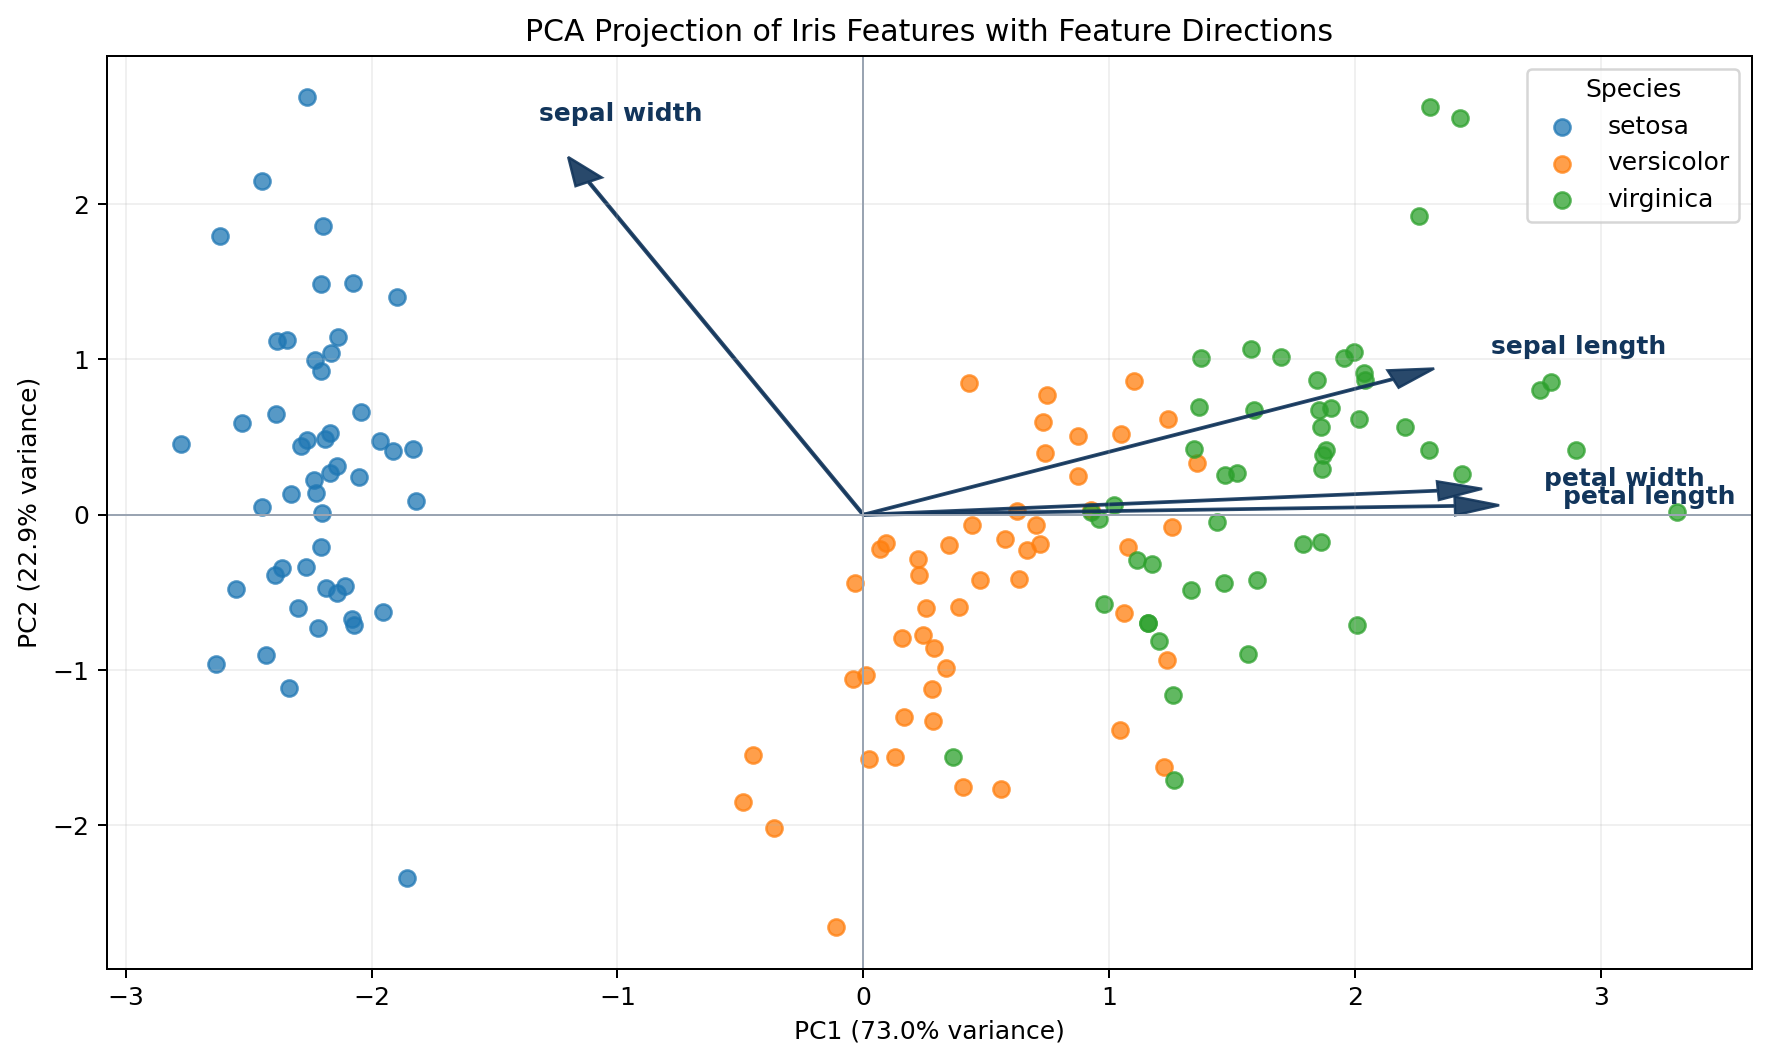
\includegraphics[height=0.76\textheight]{images/class03_pca_yellowbrick_style.png}

{\scriptsize Recreated from the `Class3_PCA.ipynb` Yellowbrick step with the same Iris PCA projection and feature directions.}
\coursefooter
\end{frame}

\begin{frame}{Where PCA helps and where it hurts}
\begin{columns}[T]
\column{0.48\textwidth}
\textbf{Helpful when}
\begin{itemize}
\item Visualizing structure
\item Reducing collinearity
\item Denoising signals
\item Speeding downstream models
\end{itemize}
\column{0.48\textwidth}
\textbf{Risky when}
\begin{itemize}
\item Stakeholders need direct feature meaning
\item Nonlinear structure dominates
\item Scaling was inconsistent
\item Drift changes the meaning of the basis
\end{itemize}
\end{columns}
\coursefooter
\end{frame}

\begin{frame}{Interpretability discussion}
\begin{itemize}
\item A component is a weighted combination of original features, not a business concept by itself.
\item High explained variance does not automatically imply high decision value.
\item Dimensionality reduction may help the model while making explanation harder.
\end{itemize}
\begin{block}{Fraud example}
The fraud dataset already contains PCA-derived variables `V1`--`V28`, so students should ask what interpretability remains when the original dimensions are hidden.
\end{block}
\coursefooter
\end{frame}

\begin{frame}{Repository connections}
\repoactivity{
\begin{itemize}
\item `notebooks/Class3_PCA.ipynb` uses Iris to build intuition and show projection plots.
\item `notebooks/Class3_PCA_Exercise.ipynb` extends the analysis to Wine.
\item `documents/FraudDetectionAsaService.pdf` describes a deployed workflow where PCA-based fields are part of a real classification task.
\end{itemize}
}
\coursefooter
\end{frame}

\begin{frame}[fragile]{Exercise anchor: Wine dataset for comparison}
\begin{lstlisting}[style=coursepython]
from sklearn.datasets import load_wine
import pandas as pd

wine = load_wine()
df_wine = pd.DataFrame(
    wine.data, columns=wine.feature_names
)
df_wine["target"] = wine.target
\end{lstlisting}
\begin{itemize}
\item `notebooks/Class3_PCA_Exercise.ipynb` starts here and is a good follow-up because Wine has more features and a less toy-like decision boundary.
\item It lets students compare PCA as a visualization tool versus PCA as a compression step before modeling.
\end{itemize}
\coursefooter
\end{frame}

\begin{frame}{From notebook to production}
\begin{itemize}
\item Fit PCA only on training data.
\item Persist the scaler and PCA object together with the model.
\item Apply the exact same transformation at inference time.
\item Recheck the basis when the distribution of inputs changes.
\item Record how many components were chosen and why.
\end{itemize}
\coursefooter
\end{frame}

\begin{frame}{Common mistakes}
\begin{itemize}
\item Running PCA before understanding the meaning of the raw features.
\item Comparing models trained on differently scaled inputs.
\item Keeping components only because the scree plot ``looks nice''.
\item Forgetting that PCA can hide bias or leakage just as easily as raw features can.
\end{itemize}
\coursefooter
\end{frame}

\begin{frame}{Technology links}
\readinglist{
\href{https://scikit-learn.org/stable/modules/decomposition.html\#pca}{scikit-learn PCA guide};\ 
\href{https://scikit-learn.org/stable/modules/generated/sklearn.decomposition.PCA.html}{PCA API reference};\ 
\href{https://scikit-learn.org/stable/modules/compose.html}{scikit-learn pipelines};\ 
\href{https://matplotlib.org/stable/}{Matplotlib documentation}.
}
\coursefooter
\end{frame}

\classclosingframe
{\begin{itemize}
\item Dimensionality reduction is useful when it improves structure, visualization, or downstream learning.
\item PCA is a transformation pipeline choice, not a universal preprocessing rule.
\item Interpretation, scaling, and deployment consistency matter as much as variance explained.
\end{itemize}}
{Use PCA when you need compact representations, denoising, or lower-dimensional plots, but keep the transformation tied to the same training-serving pipeline.}
{Class 4 turns from latent components to deliberate feature engineering: creating, encoding, scaling, and organizing variables that better represent the problem.}
{After understanding and compressing data, we make explicit design choices about the features that models and services will consume.}

\begin{frame}{Papers and materials}
\readinglist{
\href{https://link.springer.com/book/10.1007/b98835}{Jolliffe, Principal Component Analysis};\ 
\href{https://arxiv.org/abs/1309.0238}{Buitinck et al. (2013), API design for machine learning software};\ 
\href{https://www.jmlr.org/papers/volume12/pedregosa11a/pedregosa11a.pdf}{Pedregosa et al. (2011), scikit-learn};\ 
\href{https://jmlr.org/papers/volume13/bergstra12a/bergstra12a.pdf}{Bergstra and Bengio (2012), Random Search}.
}
\coursefooter
\end{frame}

\end{document}
